\chapter{树}

\begin{Def}
    连通且无圈的无向图称为无向树,简称{\bfseries树}。 一个没有圈的无向图
    称为无向森林,简称{\bfseries森林}。
  \end{Def}
  \begin{Thm}
  设$G=(V,E)$为一个$(p,q)$图,下列各命题等价:
  \begin{enumerate}
  \item $G$为树;
  \item $G$的任意两个不同的顶点间有唯一的一条路联结;
  \item $G$为连通的且去掉任意一条边则得到一个不连通的图;
  \item $G$为连通的且$q = p - 1$;
  \item $G$中无圈且$q = p - 1$;
  \item $G$中无圈且$G$中任意两个不邻接的顶点间加一条边则得到一个含有圈的图。
  \end{enumerate}
  \end{Thm}
  \begin{proof}[证明]

    $1\Rightarrow2$

    用反证法。假设图$G$中存在两个顶点$u$和$v$,在它们之间存在两条不同的路$P_1$和
    $P_2$。由于$P_1\neq P_2$,$P_1$上存在一条边$x=u_1v_1$不在$P_2$上。由$P_1$和
    $P_2$上所有的顶点和边构成的$G$的子图记为$P_1\cup P_2$, 则$(P_1\cup P_2)- x$
    是连通的。于是,$(P_1\cup P_2)-x$中存在一条$u_1-v_1$路$P$,$P+x$为$G$的一个
    圈,矛盾。

    $2\Rightarrow3$

显然,图G为连通的。设$uv$为图$G$的任意一条联结顶点$u$和$v$的边,则$uv$为联结顶点
$u$和$v$的唯一的一条路,从图$G$中去掉边$uv$之后,顶点$u$和顶点$v$之间没有路,于
是得到了一个不连通的图。

$3\Rightarrow 4$

用数学归纳法证明,施归纳于顶点数$p$。

当$p=1$时,结论显然成立。

假设当$p=k$时结论成立,往证当$p=k+1$时结论也成立。
由图$G$为连通的且去掉任意一条边则得到一个不连通的图知图$G$中一定存在一个度为1的
顶点$v$。在图$G$中去掉顶点$v$及其与之关联的边,得到图$G'$。则图$G'$为连通的且去
掉任意一条边会得到一个不连通的图,由归纳假设,图$G'$中有$k-1$条边,于是图$G$中有
$k$条边,$q=p-1$成立,定理得证。

$4\Rightarrow 5$

用反证法。假设图$G$中有圈,则去掉圈上的一条边,得到的图仍然为连通的。如果新得到
的图仍然有圈,在圈上再去掉一条边,又会得到一个新的连通的图。如此继续下去,最终会
得到一个连通的没有圈的图。由从$1$到$4$的证明知最后到的图中有$p-1$条边,这与去掉
边之前图$G$中的边数$q=p-1$矛盾。

$5\Rightarrow 6$

设图$G$有$k$个支,则图$G$中的每个支连通且没有圈。设第$i$个支中含有$p_i$个顶点,
$q_i$条边。由$1$到$4$的证明知在第$i$个支中$q_i=p_i-1$。将所有支的边数和顶点数相
加,可得$q = p-k$。于是$k=1$,从而$G$为连通的。设$u$与$v$为图$G$的任意两个不
邻接的顶点,则$u$与$v$之间存在一条路,再在$u$与$v$之间加一条边,则得到一个圈。

$6\Rightarrow 1$

设$u$和$v$为图$G$的任意两个顶点。如果$u$和$v$邻接,则$u$和$v$之间有一条路。如果
$u$和$v$之间不邻接,则在$u$和$v$之间加一条边,会得到一个圈。在该圈上将边$uv$去掉,
则得到$u$与$v$之间的一条路。这证明了$G$为连通的。
\end{proof}
  \begin{Def}
    设$G=(V,E)$为一个图,$G$的一个生成子图$T=(V,F)$如果是树,则称$T$为$G$的{\bfseries 生成树}。
  \end{Def}
  \begin{Thm}
    图$G$有生成树的充分必要条件是$G$为一个连通图。
  \end{Thm}
  \begin{Def}
    设$v$为图$G$的一个顶点,如果$G-v$的支数大于$G$的支数,则称顶点$v$为图$G$的一个{\bfseries 割点}。
  \end{Def}
  \centering
    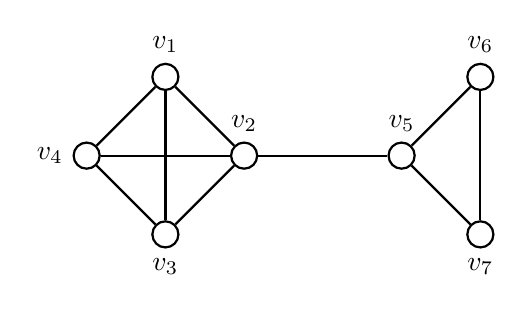
\begin{tikzpicture}[auto,
    specification/.style ={circle, draw, thick}]
   \node[specification] (A) [label=90:$v_1$] at (1,1)  {};
   \node[specification] (B) [label=90:$v_2$] at (2,0)  {};
   \node[specification] (C) [label=-90:$v_3$] at (1,-1)  {};
   \node[specification] (D) [label=180:$v_4$] at (0,0)  {};
   \node[specification] (E) [label=90:$v_5$] at (4,0) {};
   \node[specification] (F) [label=90:$v_6$] at (5,1) {};
   \node[specification] (G) [label=-90:$v_7$] at (5,-1) {};
   \draw[thick] (A) to  (B);
   \draw[thick] (B) to  (C);
   \draw[thick] (C) to  (D);
   \draw[thick] (D) to  (A);
   \draw[thick] (A) to  (C);
   \draw[thick] (B) to  (D);   
   \draw[thick] (B) to  (E);
   \draw[thick] (E) to  (F);
   \draw[thick] (F) to  (G);
   \draw[thick] (G) to  (E);
 \end{tikzpicture}  
  \begin{Thm}
    设$v$为连通图$G=(V,E)$的一个割点,则下列命题等价:
    \begin{enumerate}
    \item $v$为图$G$的一个割点;
    \item 集合$V\setminus \{v\}$有一个二划分$\{U,W\}$, 使得对任意的$u \in U$,$w \in W$,$v$在联结$u$和$w$的每条路上;
    \item 存在与$v$不同的两个顶点$u$和$w$,使得$v$在每一条$u$与$w$间的路上。
    \end{enumerate}
  \end{Thm}
  \centering
    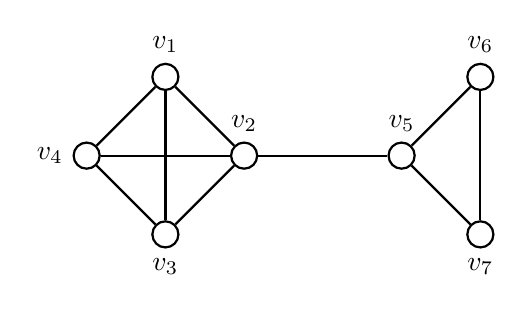
\begin{tikzpicture}[auto,
    specification/.style ={circle, draw, thick}]
   \node[specification] (A) [label=90:$v_1$] at (1,1)  {};
   \node[specification] (B) [label=90:$v_2$] at (2,0)  {};
   \node[specification] (C) [label=-90:$v_3$] at (1,-1)  {};
   \node[specification] (D) [label=180:$v_4$] at (0,0)  {};
   \node[specification] (E) [label=90:$v_5$] at (4,0) {};
   \node[specification] (F) [label=90:$v_6$] at (5,1) {};
   \node[specification] (G) [label=-90:$v_7$] at (5,-1) {};
   \draw[thick] (A) to  (B);
   \draw[thick] (B) to  (C);
   \draw[thick] (C) to  (D);
   \draw[thick] (D) to  (A);
   \draw[thick] (A) to  (C);
   \draw[thick] (B) to  (D);   
   \draw[thick] (B) to  (E);
   \draw[thick] (E) to  (F);
   \draw[thick] (F) to  (G);
   \draw[thick] (G) to  (E);
 \end{tikzpicture}  
  \begin{Def}
   图$G$的一条边$x$称为$G$的一座{\bfseries 桥},如果$G-x$的支数大于$G$的支数。
  \end{Def}
  \centering
    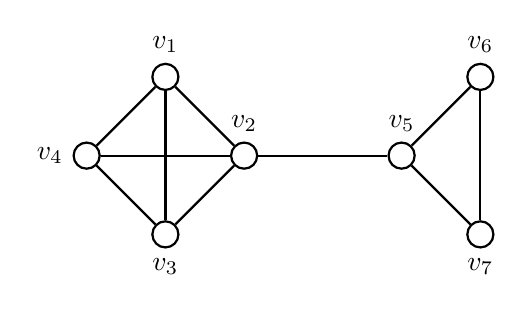
\begin{tikzpicture}[auto,
    specification/.style ={circle, draw, thick}]
   \node[specification] (A) [label=90:$v_1$] at (1,1)  {};
   \node[specification] (B) [label=90:$v_2$] at (2,0)  {};
   \node[specification] (C) [label=-90:$v_3$] at (1,-1)  {};
   \node[specification] (D) [label=180:$v_4$] at (0,0)  {};
   \node[specification] (E) [label=90:$v_5$] at (4,0) {};
   \node[specification] (F) [label=90:$v_6$] at (5,1) {};
   \node[specification] (G) [label=-90:$v_7$] at (5,-1) {};
   \draw[thick] (A) to  (B);
   \draw[thick] (B) to  (C);
   \draw[thick] (C) to  (D);
   \draw[thick] (D) to  (A);
   \draw[thick] (A) to  (C);
   \draw[thick] (B) to  (D);   
   \draw[thick] (B) to  (E);
   \draw[thick] (E) to  (F);
   \draw[thick] (F) to  (G);
   \draw[thick] (G) to  (E);
 \end{tikzpicture}  

   \begin{Thm}
    设$x$为连通图$G=(V,E)$的一条边,则下列命题等价:
    \begin{enumerate}
    \item $x$为$G$的桥;
    \item $x$不在$G$的任一圈上;
    \item 存在$V$的一个划分$\{U,W\}$,使得对任意的$u \in U, w \in W$,$x$在每一条联结$u$与$w$的路上;
    \item 存在$G$的不同顶点$u$和$v$,使得边$x$在联结$u$和$v$的每条路上。
    \end{enumerate}
  \end{Thm}
  \centering
    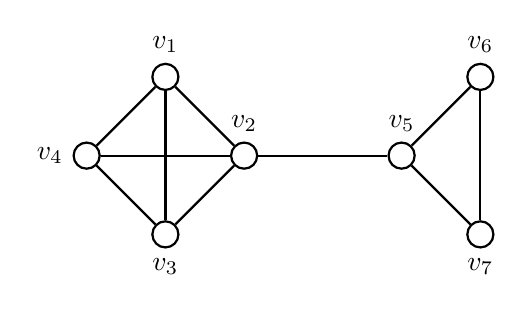
\begin{tikzpicture}[auto,
    specification/.style ={circle, draw, thick}]
   \node[specification] (A) [label=90:$v_1$] at (1,1)  {};
   \node[specification] (B) [label=90:$v_2$] at (2,0)  {};
   \node[specification] (C) [label=-90:$v_3$] at (1,-1)  {};
   \node[specification] (D) [label=180:$v_4$] at (0,0)  {};
   \node[specification] (E) [label=90:$v_5$] at (4,0) {};
   \node[specification] (F) [label=90:$v_6$] at (5,1) {};
   \node[specification] (G) [label=-90:$v_7$] at (5,-1) {};
   \draw[thick] (A) to  (B);
   \draw[thick] (B) to  (C);
   \draw[thick] (C) to  (D);
   \draw[thick] (D) to  (A);
   \draw[thick] (A) to  (C);
   \draw[thick] (B) to  (D);   
   \draw[thick] (B) to  (E);
   \draw[thick] (E) to  (F);
   \draw[thick] (F) to  (G);
   \draw[thick] (G) to  (E);
 \end{tikzpicture}  
  \begin{Def}
    设$G = (V,E)$为图,$S \subseteq E$。如果从$G$中去掉$S$中的所有边得到的图$G-S$的支数大于$G$的支数,而去掉$S$的任一真子集中的边得到的图的支数不大于$G$的支数,则称$S$为$G$的一个{\bfseries 割集}。
  \end{Def}
  \centering
    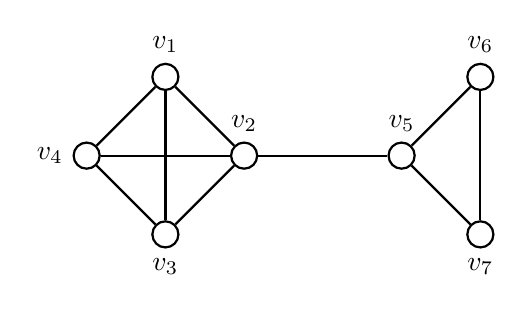
\begin{tikzpicture}[auto,
    specification/.style ={circle, draw, thick}]
   \node[specification] (A) [label=90:$v_1$] at (1,1)  {};
   \node[specification] (B) [label=90:$v_2$] at (2,0)  {};
   \node[specification] (C) [label=-90:$v_3$] at (1,-1)  {};
   \node[specification] (D) [label=180:$v_4$] at (0,0)  {};
   \node[specification] (E) [label=90:$v_5$] at (4,0) {};
   \node[specification] (F) [label=90:$v_6$] at (5,1) {};
   \node[specification] (G) [label=-90:$v_7$] at (5,-1) {};
   \draw[thick] (A) to  (B);
   \draw[thick] (B) to  (C);
   \draw[thick] (C) to  (D);
   \draw[thick] (D) to  (A);
   \draw[thick] (A) to  (C);
   \draw[thick] (B) to  (D);   
   \draw[thick] (B) to  (E);
   \draw[thick] (E) to  (F);
   \draw[thick] (F) to  (G);
   \draw[thick] (G) to  (E);
 \end{tikzpicture}  

\chapter{}
%%% Local Variables:
%%% mode: latex
%%% TeX-master: "book_chapter7"
%%% End:
